\documentclass[a4paper,10pt,english]{article}
\usepackage{mathptmx}
\renewcommand{\familydefault}{\rmdefault}
\usepackage{graphicx}
\usepackage{babel}

\usepackage{orstylet}
\makeatother
\begin{document}
\renewcommand{\figurename}{Fig.} 


\title{ONE-PAGE ABSTRACTS TITLE GIVEN IN UP TO 3 ROWS, 14 PT, BOLD, ROMAN }


\author{\uline{Author FirstAuthor}$^{1}$, Author SecondAuthor$^{1,2}$, Author ThirdAuthor
(12 point, full names)}

\maketitle

\address{$^{1}$Department of Physics, University of North Pole, Some Country
(10 point) }


\address{$^{2}$Department of Chemistry, University of South Pole, Other Country }


\rightaddress{presenter@university.com (10 point)}

This document presents how your thesis should be prepared for publishing. The abstract cannot exceed one A4 page. The size of the margins should be chosen as follows: top, bottom, left and right -- 20mm.

The format to be used is as follows: (i) the abstract title (Roman font, Bold, 14pt, All Caps, Centered) should be no more than 3 rows in length (centered); no empty line after the title; (ii) the authors’ names (Roman font, Normal, 12pt, Centered) should be listed as shown in the above example, with the presenting author’s name underlined; please write unabbreviated names; empty 10pt line break after the author list; (iii) author affiliations (Roman font, Normal, 10pt, Centered), indicated using numerical superscripts; (iv) email address of the presenter.

The body text of the abstract (Roman font, 10pt) should be both left- and right-justified. The first line of each paragraph should be indented by 0.75 cm, except of the figure caption and references. Do not add spaces/empty lines between paragraphs. The references \cite{key-1} are cited in the text in the order they appear. The reference list should use the format shown below.

Do not use fonts, smaller than 7 pt in figures (for example Fig.~\ref{fig:Example_figure}), graphs and tables or anywhere else in the document. All abbreviations should be fully introduced at their first appearance in the text.

\begin{figure}[h]
\begin{centering}
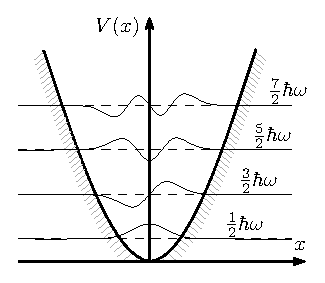
\includegraphics{figure}
\par\end{centering}

\caption{\label{fig:Example_figure}First four wavefunctions of quantum harmonic
oscillator.}
\end{figure}
Numbered equations are placed on a separate line and centered. The mathematical symbols are typeset in standard notation: functions and variables in italic, standard functions ($\sin$, $\exp$, ...), mathematical constants ($\mathrm{e}=2.71828...$; $\mathrm{i}^2=-1$; etc.), differential and other symbols in a regular (upright) mode. When referring to the equations in the text, enclose their numbers in parentheses, e.~g., Eq.~(\ref{eq:Maxwell}):

\begin{equation}
\mathrm{rot}\:\mathrm{rot}\:\hat{E}(\vec{r},t)+\left(\frac{\imath}{c}\right)^{2}\frac{\mathrm{d}^{2}}{\mathrm{d}t^{2}}\hat{E}(\vec{r},t)=-\frac{4\pi}{c}\frac{\mathrm{d}^{2}}{\mathrm{d}t^{2}}\hat{P}(\vec{r},t).\label{eq:Maxwell}
\end{equation}
Write the link to the references in angular brackets \cite{key-1}. The list of the references should be written in 8 pt. Times New Roman font. 

The abstract book will be printed in greyscale (color online). Please consider it when preparing the figures to avoid ambiguities in greyscale-printed book. The quality of photos should be at least 150 dpi.

\begin{thebibliography}{References}

\bibitem{key-1}K. Melcher, L.-M. Ng, E. Zhou et al., A gate-latch-lock
mechanism for hormone signaling by abscisic acid receptors, Nature
\textbf{462}, 602-608 (1990).

\bibitem{key-4}M. A. Green, \textit{High Efficiency Silicon Solar
Cells} (Trans. Tech. Publications, Switzerland, 1987).

\bibitem{key-2}J. Belovickis, Acoustooptic interaction of leaky surface
acoustic waves in YX-LiTaO3 crystals, 54th scientific conference for
young students of physics and natural sciences Open Readings 2011,
ISSN 2029-4420, Vilnius University, 103-104 (2011).\end{thebibliography}

\end{document}
